\chapter{Primer korišćenja \textit{Elastic stack}-a}
U ovom poglavlju će biti opisana implementacija sistema koji je iskorišćen kao jedan od mnogih primera korišćenja \textit{\textbf{Elastic stack}} alata. Sistem koji je implementiran ima ulogu obrađivanja podataka mrežnog saobraćaja u realnom vremenu, kroz njihovo parsiranje, transfomaciju, nadogradnju, skladištenje i vizuelizaciju. Kompletna implementacija je ostvarena korišćenjem odgovarajućih komponenti \textit{\textbf{Elastic stack}}-a i kontejnarizovana u okviru \textit{\textbf{Docker}} \cite{docker} kontejnera uz pomoć \textit{\textbf{Docker compose}} alata \cite{docker-compose}. 

\section{Arhitektura implementiranog sistema} 
Kompletna arhitektura sistema je prikazana na dijagramu \ref{diagram:arhitektura-sistema-primera-koriscenja}. U okviru sistema se mogu prepoznati već opisane komponente iz prethodnog poglavlja.

\begin{figure}[H]
    \centering
    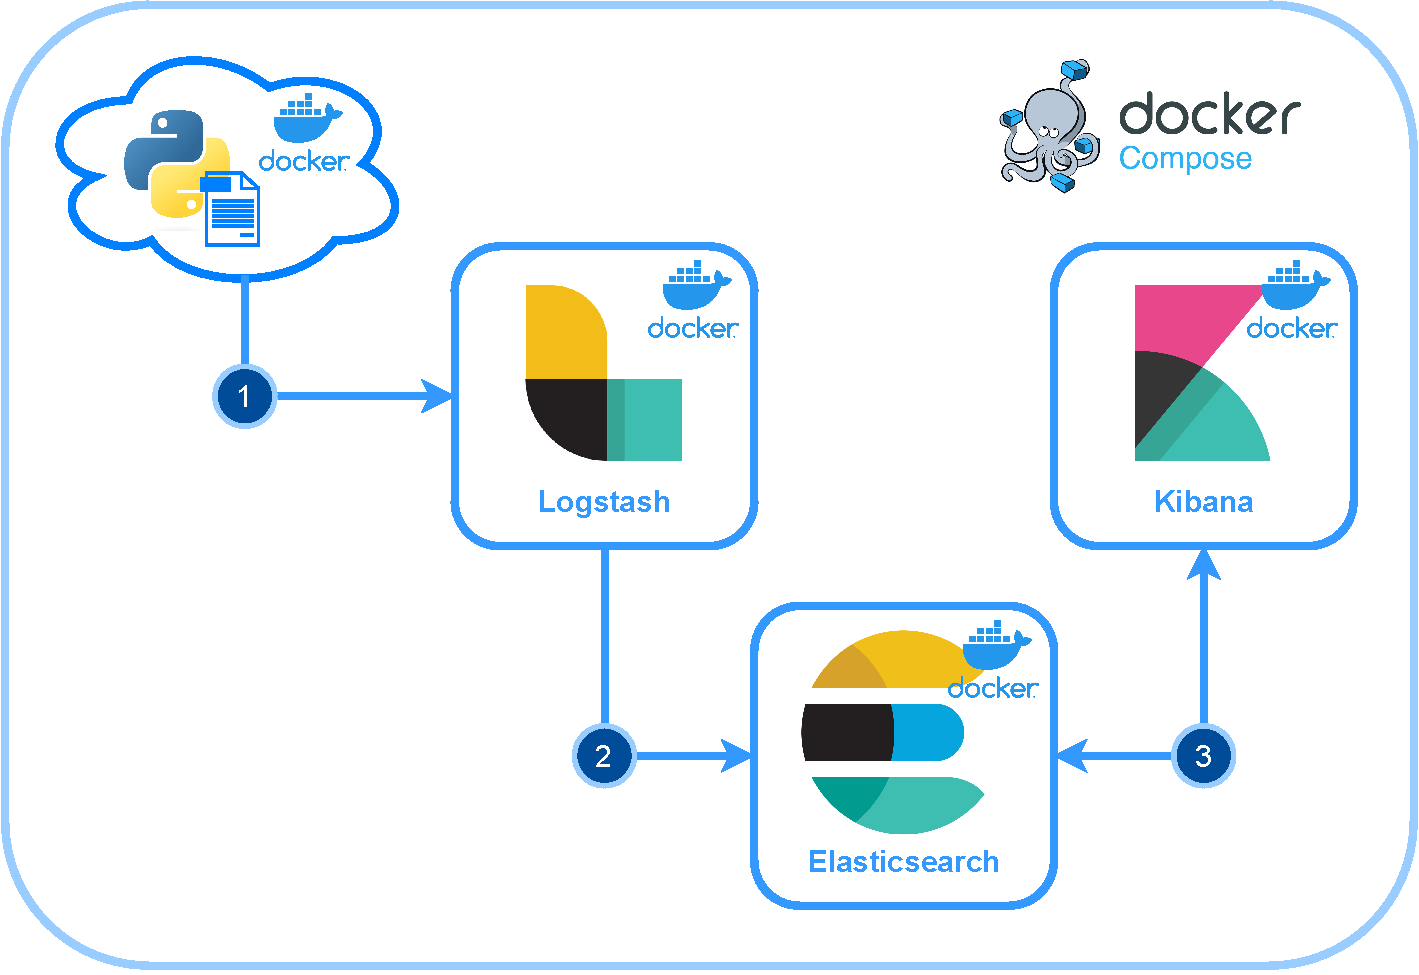
\includegraphics[width=\columnwidth]{images/Impl-arch.pdf}
    \caption{\textit{Dijagram arhitekture sistema}}
    \label{diagram:arhitektura-sistema-primera-koriscenja}
\end{figure}

\par
Podaci o mrežnom saobraćaju su simulirani kratkom \textit{\textbf{Python}} skriptom koja čita podatke iz dataset-a \cite{dataset}, povezuje se na \textit{\textbf{Logstash}} ulazni dodatak uz pomoć \textit{TCP} konekcije i šalje sadržaj u određenim vremenskim intervalima. Ovim se ostvaruje unošenje sirovih podataka za obrađivanje u realnom vremenu, što je označeno kao \textbf{korak 1} na dijagramu. \textit{\textbf{Logstash}} komponenta je zadužena za prihvatanje sirovih podataka u sistem. U okviru pokrenutog toka podataka, \textit{\textbf{Logstash}} parsira sirove podatke, unosi u njih semantiku, vrši njihovo obogaćivanje i tako obrađene podatke šalje na \textit{\textbf{Elasticsearch}}, što je označeno kao \textbf{korak 2} na dijagramu.

\par
Komponenta \textit{\textbf{Elasticsearch}} je zadužena za indeksiranje, skladištenje i pretraživanje podataka na osnovu polja koja je \textit{\textbf{Logstash}} kreirao. Ovi podaci su dostupni \textit{\textbf{Kibana}} komponenti, koja može da na osnovu njih kreira vizualnu reprezentaciju iz koje se mogu izvući nova znanja, odnosno zaključci. Komunikacija između alata \textit{\textbf{Kibana}} i \textit{\textbf{Elasticsearch}} je dualna, označena kao \textbf{korak 3} na dijagramu, s obzirom da se dijagrami koji se kreiraju u okviru alata \textit{\textbf{Kibana}} skladište u okviru \textit{\textbf{Elasticsearch}} instance.

\par
Uzeći u obzir performanse računara na kome je pokrenut ovaj sistem, nijedna komponenta nije replicirana. Svaka komponenta ima jednu instancu koja je pokrenuta u svom kontejneru i komunikacija se odvija isključivo direktnom mrežnom komunikacijom, odnosno ne postoje balanseri opterećenja. U još realnim primeru, instance bi bile replicirane i pokrenute sa mnogo više alocirane memorije u okviru \textit{JVM}-e, kao i činjenica da bi postojali balanseri opterećenja za različite instance \textit{\textbf{Logstash}} komponente.

\section{Konfiguracioni fajlovi sistema}
Svaka od komponenti sistema je pokrenuta u okviru sopstvenog \textit{\textbf{Docker}} kontejnera, a za pokretanje sistema se koristi \textit{\textbf{Docker compose}} alat, te je celokupan sistem moguće konfigurisati u okviru par fajlova i pokrenuti samo jednom komandom \mintinline{shell-session}{docker-compose up}. Sadržaj \textit{\textbf{docker-compose.yml}} fajla se nalazi na isečku \ref{code:docker-compose}.

\begin{listing}
\inputminted[
    frame=single,
    linenos,
    fontsize={\fontsize{5.5}{5.5}\selectfont},
    breaklines
  ]{yaml}{kod/docker-compose.yml}
  \caption{\textit{Konfiguracija \textbf{docker-compose.yml} fajla}}
  \label{code:docker-compose}
\end{listing}

\par
Sa isečka \ref{code:docker-compose}, u okviru linija 4-27 možemo primetiti servis pod nazivom \textit{\textbf{setup}}, koji je odgovoran za konfigurisanje određenih parametara instanci \textit{\textbf{ELK stack}}-a. Ovaj servis se pokreće nakon što je servis \textit{\textbf{Elasticsearch}} podignut i izvršava \textit{\textbf{setup}} skriptu. \textit{\textbf{Elasticsearch}} servis je konfigurisan u okviru linija 29-47. Za ovaj servis su otvoreni portovi 9200 i 9300 čija funkcija je upisana u sekciji \ref{subsection:osnove-elasticsearch-a}. Parametri \textit{JVM}-e su prosleđeni na liniji 42 i to sa minimalno neophodnom memorijom od 512MB.

\par
\textit{\textbf{Logstash}} servis je konfigurisan u okviru linija 49-71 i to sa otvorenim portovima 5044, 50000 i 9600. Port 5044 se koristi za \textbf{Beats} ulazni dodatak, dok je port 50000 otvoren za \textit{TCP} i \textit{UDP} ulazne dodatke. Port 9600 se koristi za komunikaciju sa \textit{\textbf{ELK stack}}-om. Ova komponenta takođe ima minimalne memorijske parametre za izvršavanje u \textit{JVM}-i. U okviru linija 73-88 je konfigurisan servis \textit{\textbf{Kibana}}, koji je pokrenut na portu 5601, što je standardni port za ovu komponentu.

\par
Konfiguracija svih komponenti, osim \textit{\textbf{Logstash}}-a je standardna konfiguracija koju preporučuje kompanija Elastic u svojoj dokumentaciji, odnosno dostupna na github repozirotijumu \cite{elk-docker-compose-repo}.

\par
\textit{\textbf{Logstash}} konfiguracija je izmenjena kako bi se prilagodila ovom primeru. Odnosno tok podataka je konfigurisan na sledeći način (isečak \ref{code:logstash-pipeline}).

\begin{listing}
\inputminted[
    frame=single,
    linenos,
    fontsize={\fontsize{5.5}{5.5}\selectfont},
    breaklines
  ]{js}{kod/logstash.conf}
  \caption{\textit{Tok podataka \textbf{Logstash.conf}}}
  \label{code:logstash-pipeline}
\end{listing}

\par
Ulazna etapa toka podataka je konfigurisana u okviru linija 1-6. U okviru nje je definisan jedna ulazni dodatak, odnosno \textit{TCP}, koji osluškuje na portu 5000 i koristi \textit{\textbf{plain}} kodek za dekodiranje ulaznih podataka. Ovaj kodek podržava tekstualne podatke, odnosno vrši konverziju iz bajtova u string i podrazumevano koristi \textit{utf-8} format.

\par
Obrađivanje podataka se odvija u okviru filter etape definisane na linijama 8-80. S obzirom da se dodaci filter etape izvršavaju sekvencijalno, redosledom kojim su napisani, prvi koji se izvršava jeste \textit{\textbf{grok filter dodatak}}. U okviru njega se iz polja \textit{"message"}, koje predstavlja sadržaj ulazne etape, vrši parsiranje delova poruke i njihov upis se vrši u odgovarajuća polja pridružena šablonu. Takođe, standardna konfiguracija koju ima svaki dodatak jeste mogućnost ubacivanja tagova, odnosno polja, kao i \textit{target} polje koje precizira mesto u okviru događaja, koji se trenutno obrađuje, gde će se smestiti rezultat dodatka. U okviru linije 19 je postavljen uslov da ukoliko se na polju \textit{gen} događaja, koji se obrađuje, ne nalazi vrednost \textit{network-traffic}, filter etapa se završava.

\par
Za događaje koji su označeni kao \textit{network-traffic}, sledi obrada u okviru linija 20-78. S obzirom da su navedeni dodaci već objašnjeni, trebalo bi da je jasno šta se u pozadini dešava sa događajem. U okviru linija 20-23 se izvršava \textit{\textbf{http filter dodatak}}, koji prosleđuje \textit{IP} adresu izvorišta kako bi proverilo njenu reputaciju, koristeći javni \textit{API} dostupan na \textit{endpoint}-u u okviru linije 21. Rezultat se smešta u odgovarajuće ugnježdeno polje događaja. S obzirom da se upisuje string vrednost u polje, u okviru linija 24-27 se ovo polje parsira i na njegovo mesto dolazi \textit{JSON}, odnosno vrednost tipa \textit{hash}, koje sadrži odgovarajuća polja. Identična logika se izvršava i za odredišnu \textit{IP} adresu, u okviru linija 29-36.

\par
Na linijama 38-41 i 43-45 se pomoću \textit{\textbf{geoip filter dodatka}}, ispituju podaci o geo-protornim informacijama izvorišne i odredišne \textit{IP} adrese, respektivno. Nakon toga se za svaku od njih, u zavisnosti od toga da li je geo-prostorna pretraga bila uspešna, pripremaju polja za povratnu \textit{DNS} pretragu, koristeći filter dodatak \textit{\textbf{mutate}} u okviru linija 48-55 za izvorišnu, odnosno 57-64 za odredišnu \textit{IP} adresu.

\par
Konačno, ukoliko se radi o uspešnim geo-prostrnim vrednostima, vrši se povratna \textit{DNS} pretraga, uz pomoć \textit{\textbf{dns filter dodatka}} i vrednost pripremljenih polja se zamenjuje sa rezultatima pretrage, u okviru linija 66-70 za izvorišnu, odnosno 73-78 za odredišnu \textit{IP} adresu. Ovime je filter etapa okončana.

\par
U okviru izlazne etape, podaci koji sadrže \textit{network-traffic} vrednost u okviru \textit{gen} polja bivaju upisani na \textit{\textbf{Elasticsearch}} instancu, koristeći istoimeni izlazni dodatak. Specifična stvar jeste dobra praksa indeksiranja, na liniji 88, gde se indeksi grupišu na osnovu datuma, po mesecu kada su generisani. Time se olakšava dalja analiza skladištenih dokumenata. Paralelno sa ovim se izvršava i neobavezan \textit{\textbf{izlazni dodatak stdout}} za ispis na standardni izlaz, koristeći \textit{\textbf{enkoder rubydebug}}.

\section{Vizuelizacija podataka}
Nakon što je komponenta \textit{\textbf{Logstash}} uspešno obradila podatke i upisala ih u \textit{\textbf{Elasticsearch}} komponentu, podaci su dostupni alatu \textit{\textbf{Kibana}} za njihovu vizuelizaciju. Za vizuelizaciju je odabrano prikazivanje geo-prostornih koordinata, s obzirom na filter etapu \textit{\textbf{Logstash}} toka podataka, te su podaci predstavljeni na svetskoj mapi, kao lokacije gde su se nalazili najbliži mrežni centri iz kojih su slati paketi. Odnosno, kreiran je pogled tipa mapa, na kome su ilustrovani podaci. Vizuelizacija podataka je prikazana na slici \ref{screenshot:vizuelizacija-podataka-na-mapi}.

\begin{figure}[H]
    \centering
    \hspace*{-0.1\columnwidth}\frame{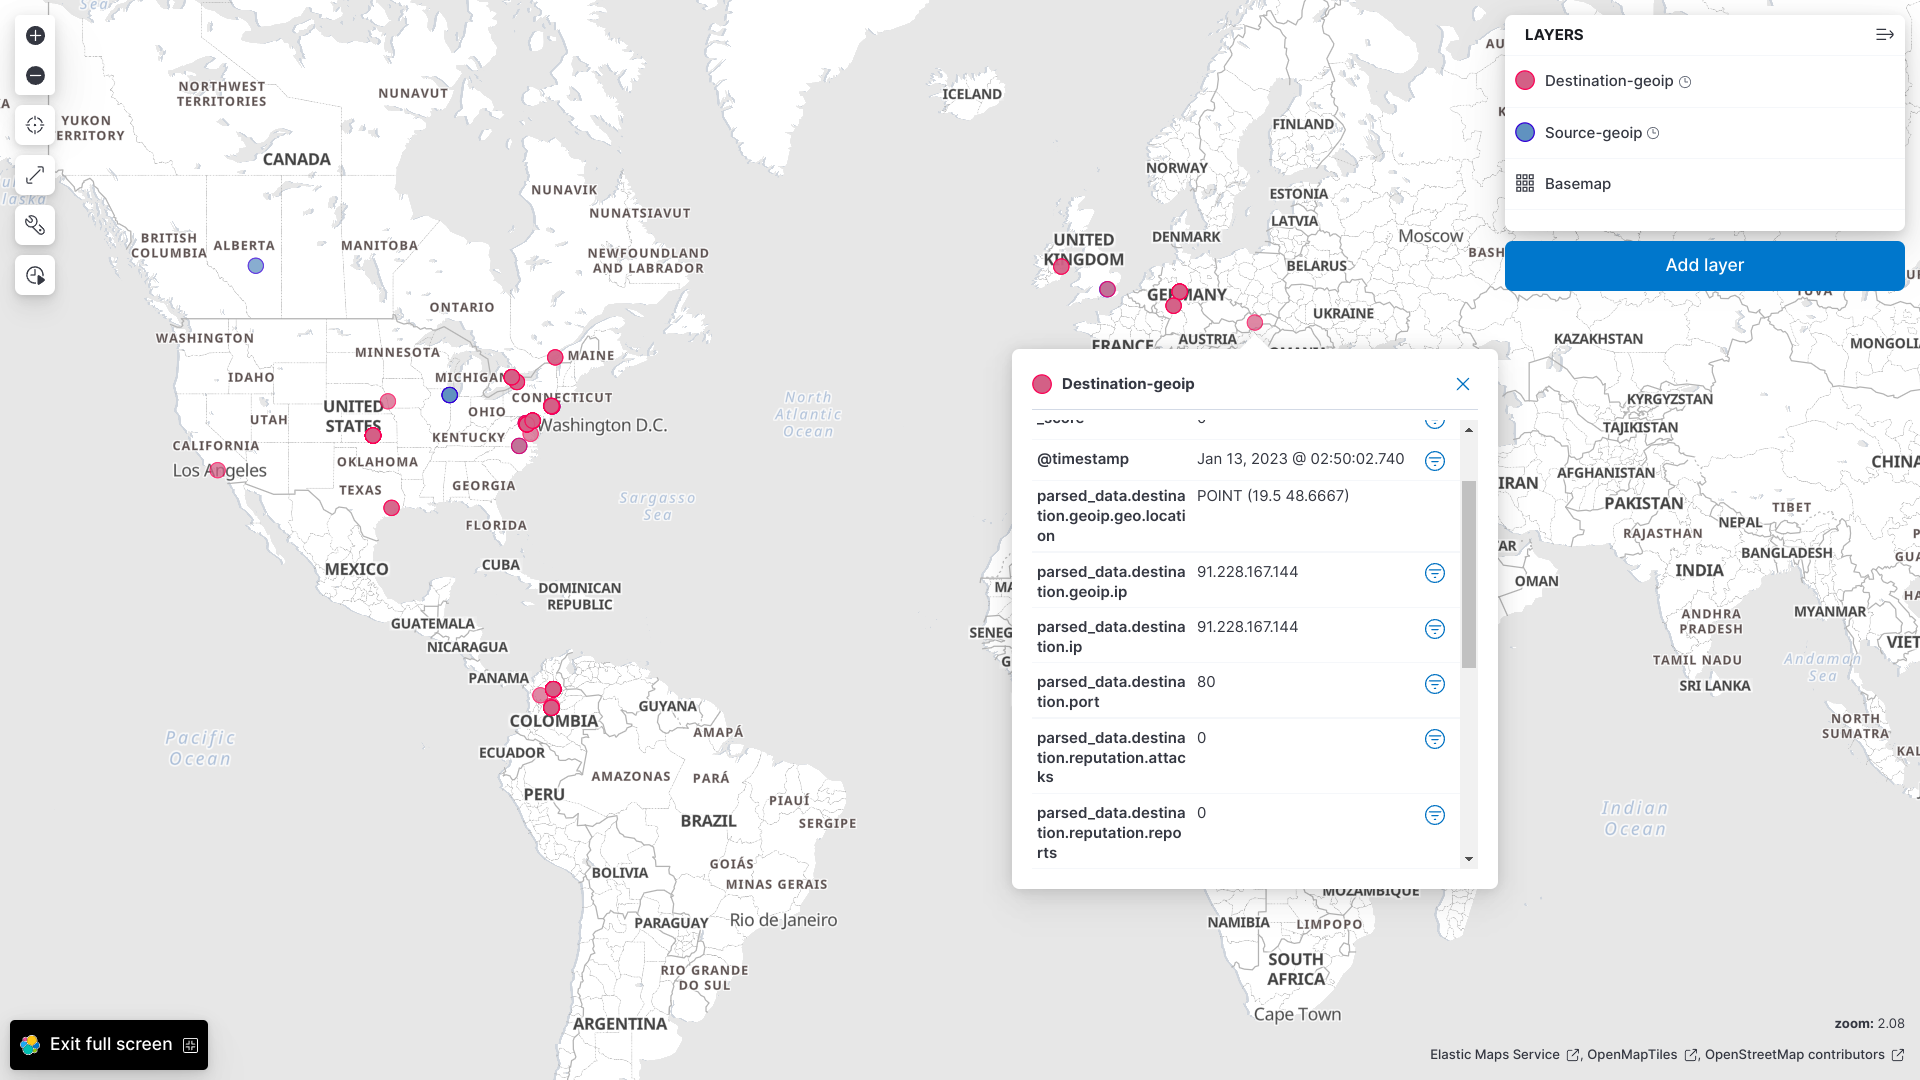
\includegraphics[width=1.2\columnwidth]{images/Screenshot from 2023-01-13 18-34-22.png}}
    \caption{\textit{Vizuelizacija podataka uz pomoć alata \textit{\textbf{Kibana}}}}
    \label{screenshot:vizuelizacija-podataka-na-mapi}
\end{figure}

\par
Ovde je moguće koristiti \textit{\textbf{KQL}} jezik za dodatno filtriranje podataka sa mape, odnosno prelazeći preko lokacija na mapi, prikazuje se \textit{tooltip} kao na slici \ref{screenshot:vizuelizacija-podataka-na-mapi}, koji pruža kratak uvid u bitnija polja skladištenih dokumenata.